 \begin{figure}[!ht]
	\begin{center}
		\makebox[\textwidth]{
			\centering
			\captionsetup{width=0.5\linewidth}
			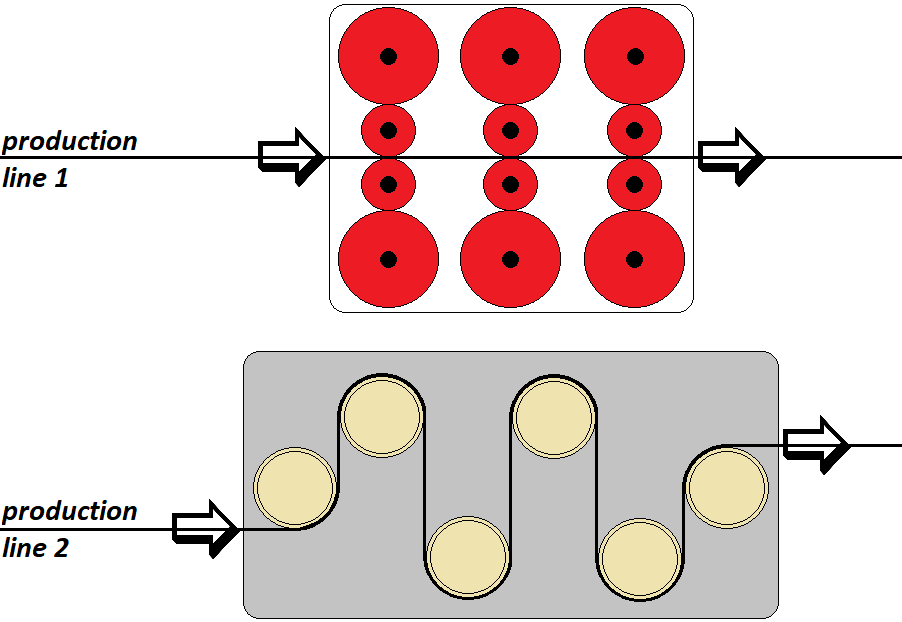
\includegraphics[width=0.9\linewidth]{../images/introduction-hypothetical_constraints.png}}
		\caption{Different Categories of Production Events Handling. The hot rolling mill presses the metal slabs with red rollers positioned in production line 1. The unit in production line 2, pickling tank full of acid coloured in grey, treats the metal surface of the slabs.
		}
		\label{figure-hypothetical_constraints}
	\end{center}
\end{figure}